\chapter{TieSim}
\label{chap:tiesim}

Clearly VR is an advanced technology, and every day more and more applications are being developed targeting it as a platform. Yet, the majority of these applications are inherently video games built and targeted for entertainment. Of course this is to be assumed, since Oculus VR said themselves on their original Kickstarter that they wanted to build the first immersive VR headset for video games. Since the release of the DK1, and well into the life cycle of the DK2, the vast majority of applications built for these HMDs have been video games. In the end, video games are driving core development and adoption of VR, but there still must exist a space for educational applications.

For this reason, part of this research consisted of delving into the development process of building an immersive VR application for educational purposes. More specifically, a program called TieSim was built which aimed to create a learning environment where a user could interact with a stationary robot, and learn how to tie a men's neck tie on said robot. The reason this task was chosen was because learning to tie a necktie is a simple task which can be taught in 30 minutes or less. Moreover, TieSim's overall goal is to link the concepts of competency based learning with a VR application. Additionally, Chapter 5 explores the idea and realization of a proposed study in which a completed version of TieSim could be used on human test subjects to see if the skill was taught effectively and successfully. The rest of this chapter explores the technical details behind TieSim, including the hardware and software choices. As well, this chapter explores the hardware choice which ultimately hindered the advancement of development, and what a future student might be able to work on to get TieSim fully functional.

\section{Project Overview}
\label{sec:project}

The concept behind TieSim is simple, TieSim is an immersive VR simulation which places the user in front of a stationary figure so that the user can learn to tie a necktie onto the figure. Teaching can be accomplished in a variety of ways, many of which can be intertwined. The methods currently in place in the simulation involve a massive monitor-like wall that sits in the user's foreground. On this wall a series of large picture and text based instructions guide the user through a series of nine simple steps in learning how to tie a half-Windsor knot. 

Another technique which could be employed would be to hire a voice actor who could give professional quality voice instructions to accompany the visuals. For the purposes of early TieSim development, a voice actor was not employed primarily due to lack of funds, but one could be hired relatively cheaply on a site such as fiver where users offer on demand freelance skill work.

The setting of the simulation takes place in a vastly open room with no walls or ceiling in sight, Figure~\ref{figure:f_kyle} demonstrates the opening scene with the user's hands out in front of them. The floor consists of a tiled pattern which extends past the field of vision. The user is placed in the seemingly center of the room, where they are found sitting at an empty desk. As mentioned, in the user's foreground is the instruction monitor, which at first prompts the user with a description of their scenario. Finally, sitting on top of the desk is a robot named Kyle who sits wearing a men's necktie. The user will learn to tie the necktie onto Kyle. 

\begin{figure}
  \centering
  %\begin{picture}
  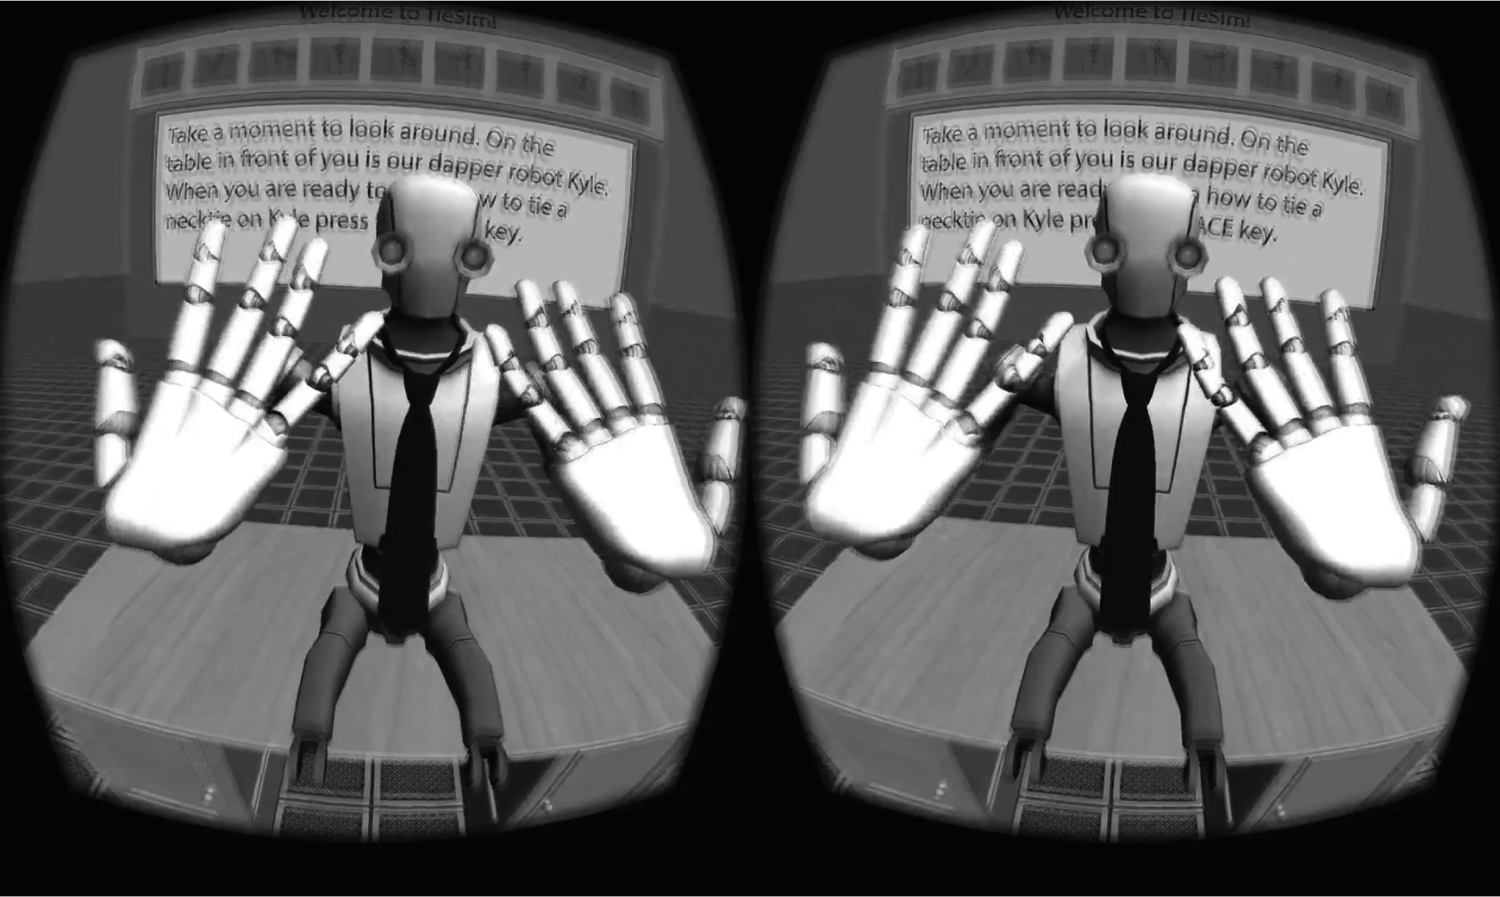
\includegraphics[scale=.55]{img_kylehands}
  %\end{picture}
  \caption{Screenshot of TieSim running with the user's hands in scene.}
  \label{figure:f_kyle}
\end{figure}
%Figure~\ref{figure:f_dk1}

The overall development production for TieSim reached near completion throughout the work done during this research, however, due to a hardware limitation it was not completed in full. More details can be found in the following section on Hardware.

\section{Hardware}
\label{sec:hardware}

A discussion on TieSim's hardware must, of course, start with the HMD. At the beginning of development, the most recent HMD available on the market was the Oculus Rift DK2, and as such it was used for this project. For a more in depth discussion on the DK2 hardware specifications see Chapter 2.2: Current VR Development. 

Besides the VR hardware, another piece of hardware known as the Leap Motion V2 was used significantly throughout development. The Leap Motion serves as an alternate input device from a mouse and keyboard, and is technically a piece of AR hardware. Essentially, the Leap Motion is a small USB device which uses two monochromatic IR cameras and three infrared LEDs to observe a hemispherical area up to a meter above the device. In this observation area the device is used to track hand and tool movements which can then be accurately modeled in a variety of development environments. Normally the Leap Motion functions by lying face up on a desktop surface; however, for the purposes of this product the Leap Motion was mounted onto the DK2 facing outwards. Further, when mounted onto the DK2 the field of views (FOVs) of both devices collide nicely, as seen in Figure~\ref{figure:f_fov}, and allow both to work together without any gaps in FOV.

\begin{figure}
  \centering
  %\begin{picture}
  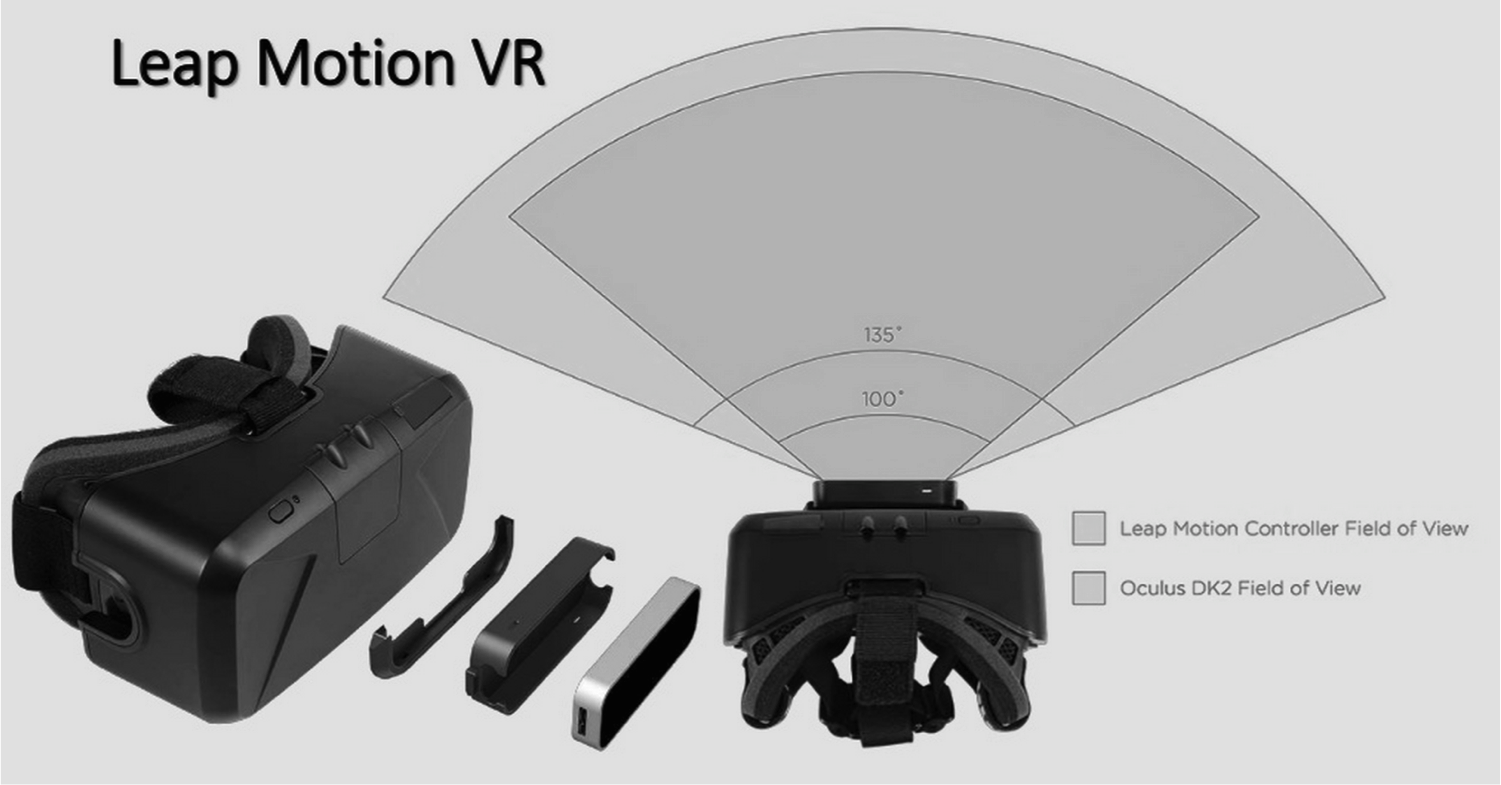
\includegraphics[scale=.55]{img_fov}
  %\end{picture}
  \caption{Visual reference of the Leap Motions and DK2's colliding FOVs.}
  \label{figure:f_fov}
\end{figure}
%Figure~\ref{figure:f_dk1}

For this project the most obvious use of the Leap Motion in conjunction with the DK2 would be to use the device for primary input in the simulation. The Leap motion provides a more natural method of input, especially when considering the task at hand. Further, using an AR input device like the Leap Motion greatly increases the sense of presence a user experiences in VR. This proved to be the case from the author's anecdotal evidence in which having a model mapped to one's actual hand movements in VR space tended to help ease the transition into VR and reduce the disconnect experienced with the emerging technology. Ultimately, the Leap Motion was a natural choice for this project. However, its choice was perhaps what ended up being the largest setback of the entire development progress (see section 4.4: Development Obstacles).

\section{Software}
\label{sec:software}

When working with VR there are only a few choices for software suites to work in. For starters, every major software suite available is first and foremost a game development engine, and of these suites there are two major choices, each with their own advantages and disadvantages. The first engine available is the newly open-sourced Unreal Engine 4 with built in Oculus Rift support. At the beginning of this project, however, Unreal Engine 4 was not available for free. It would have been considered except for its cost. Unreal Engine's biggest draw is that it is a AAA-quality engine capable of producing stunning applications with top-of-the-line graphics and systems. Of course, these great features come with an immense learning curve.

The other game engine option to consider for VR development is Unity3D. This is the engine with which TieSim was created, partially because it is the engine the author is most familiar with, and also for other key advantages the engine has over Unreal. For starters, Unity3D has less of a learning curve, and it is incredibly easy to get working quickly within its simple workspace. As well, Unity3D offers drag and drop Oculus Rift support, and it tends to be the go-to engine for VR development. Normally the largest downside to using Unity3D is its hefty license fee; however, this project qualified for an educational license which is far more reasonably priced. More discussion will follow on working with Unity3D as it was the suite chosen for this project, yet it should be noted that although Unreal Engine was not chosen for this project, it is an equally viable engine to use for VR development. 

Overall working within Unity3D is perhaps its largest draw because it is undeniably simple as seen in Figure~\ref{figure:f_unity}. Beyond this aspect, Unity3D offers a variety of scripting languages to work with, namely Javascript, C\#, and Boo Script. For TieSim, C\# was chosen as the scripting language because of its robustness over the other two choices available, and the author's familiarity with the language. As well, both Leap Motion and Oculus Rift allow scripts to access their device APIs, and allow for customizable behavior inside simulations. For Leap Motion a variety of languages can be used, namely Javascript and C\#, and for Oculus Rift C\# is the primarily used language support. Thus C\# was a fitting language to use as it allowed communication inside Unity3D with both the Oculus Rift and Leap Motion, and moreover overall scene interaction.

\begin{figure}
  \centering
  %\begin{picture}
  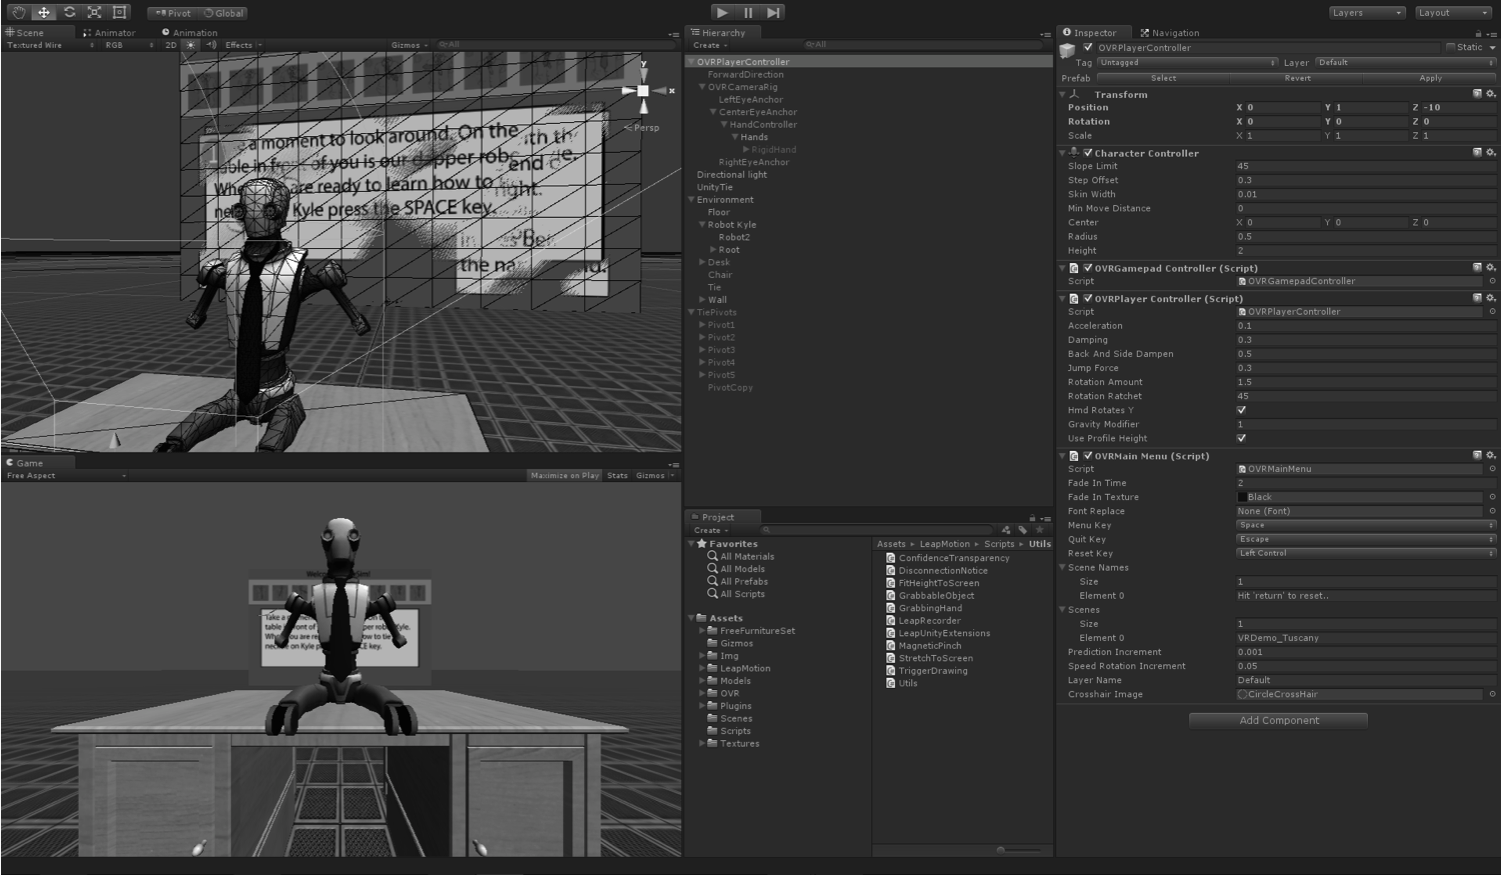
\includegraphics[scale=.55]{img_unity}
  %\end{picture}
  \caption{Screenshot of TieSim's Unity3D development environment.}
  \label{figure:f_unity}
\end{figure}
%Figure~\ref{figure:f_dk1}

An additional software suite was used for the purposes of 3D modeling the tie model used in the simulation. The 3D modeling program Blender was used, as it is an open source suite with ample documentation.

Finally, TieSim is first and foremost an open source project under the MIT educational license. All of the source code for the project is available through Git and hosted via GitHub under the author's account at the following URL: https://github.com/cleebp/TieSim. As well, all of the most up to date code as of writing has been included at the end of this work on a DVD. The purpose of making this project open source was primarily because the author recognizes that many improvements can be made to this application (see section 4.5 Results and Conclusions), and by making TieSim open source, anyone in the world can contribute to the development of the project as a public good.

\section{Development Obstacles}
\label{sec:obstacles}

Like all ambitious software projects, development of TieSim was met with its fair share of obstacles. For starters, before working on TieSim the author had little to no experience working with Oculus Rift development, and had never worked with Leap Motion hardware. As such, development was as much a learning experience as it was actual progress. This being said, development did progress fairly competently with the help of online resources, and some of the more outstanding obstacles have been listed below. Yet, by far the largest obstacle encountered in development of TieSim was ultimately working with the Leap Motion hardware. 

To begin with, online resources for working with Leap Motion could be best described as scarce. Even the official documentation for the hardware's API is lackluster, seemingly because a major API rewrite occurred between the release of the V1 hardware and the V2 hardware. Much of the original API still remains in use, and these documents are fairly well documented, yet almost all of the now existing API used by the V2 is completely undocumented. This disconnect becomes even more apparent when following the tutorials supplied on the Leap Motion website, which all use the original API and as such don't work within the existing hardware and firmware. For these reasons, working with Leap Motion was an incredible pain, and most internet searches for specific problems met with little to no results.

Additionally, Leap Motion ended up crippling development progression due to its lack of proper integration with Unity3D objects. As mentioned in Section 4.3, the 3D modeling program Blender was used to model a simple tie to be used as the core interaction object for TieSim. Needless to say, interaction with this object was critical for development progression, yet it was impossible to interact with this custom modeled object using the Leap Motion as input. The bulk of development time was spent trying any possible solution to this problem, however, it became clear that Leap Motion would halt all further development of TieSim (see section 4.5: Results and Conclusions).

\section{Results and Conclusions}
\label{sec:results}

Ultimately, TieSim's development was completely sidetracked due to the limitations of the Leap Motion hardware (see section 4.4: Development Obstacles), and as such TieSim is currently in an unfinished state. That being said, it should be noted that the basic systems necessary for a fully functional TieSim have been developed and are integrated into the application. While there currently is no way to use input to interact with the 3D modeled tie, the majority of the simulation's scene has been built and is convincingly real. As TieSim currently stands, anyone with a DK2 can run the simulation's executable and will be thrown into the scene (see section 4.1: Project Overview). 

Further development of this simulation is obviously a must, and the most direct way to pursue future development would begin with finding an alternative to using the Leap Motion for input. One could revert to using a standard gaming controller or mouse and keyboard layout; however, there are a myriad of new and exciting AR input devices constantly under new development. Migration to a different AR device that supports more minute interaction with objects in Unity3D is critical. Once a new input hardware has been chosen it should be able to be easily integrated into the existing project space. Since the systems for the sequential instructions are in place, development would need to focus on how to integrate with maneuvering the tie in order to trigger events which would advance instruction and alert the user. 

These are not small development goals, and would take a significant amount of time. As well, although not essential, prior experience working with these technologies would be a bonus. With the project being completely open source, it is possible someone would take up these development goals, or alternatively a future honors student at Appalachian State could focus their own thesis work on continuing the development of TieSim.